% ---------------------------------------          Preamble
\documentclass[
	fontsize=12pt,
	paper=a4,
	twoside=false,
	numbers=noenddot,
	plainheadsepline,
	toc=listof,
	toc=bibliography
]{scrartcl}

\usepackage[english]{babel} 

\usepackage{amssymb}
\usepackage{amsmath}
\usepackage{array}

\usepackage{placeins}
\usepackage{float}

\usepackage{graphicx}
\restylefloat{figure}
\usepackage{caption}
\usepackage{subcaption}
%\usepackage{subfigure} 
\usepackage{tikz}

%\usepackage{pdfpages} % insert images saved as pdf

% pseudo algorithms
\usepackage[ruled,vlined]{algorithm2e}

% lscape.sty Produce landscape pages in a (mainly) portrait document.
\usepackage{lscape}

\usepackage{hyperref}

\setlength{\parindent}{0pt}

\usepackage[sort, numbers]{natbib}
% ---------------------------------------          New commands
%\newcommand{\argmin}{\operatornamewithlimits{argmin}}
\def\argmax{\mathop{\rm argmax}}						% argmax
\def\argmax{\mathop{\rm argmin}}						% argmin
\def\median{\mathop{\rm median}} 						% median
\def\dist{\mathop{\rm dist}} 						    % dist

\makeatletter
\providecommand\phantomcaption{\caption@refstepcounter\@captype}
\makeatother


\usepackage{array}
\newcolumntype{L}[1]{>{\raggedright\let\newline\\\arraybackslash\hspace{0pt}}m{#1}}
\newcolumntype{C}[1]{>{\centering\let\newline\\\arraybackslash\hspace{0pt}}m{#1}}
\newcolumntype{R}[1]{>{\raggedleft\let\newline\\\arraybackslash\hspace{0pt}}m{#1}}


\usepackage{xcolor} 
\newcommand\ToDo[1]{\textcolor{red}{#1}} 

% ------------------------------------------------------------------------------------------------------------
% ------------------------------------------------------------------------------------------------------------
% ------------------------------------------------------------------------------------------------------------

\begin{document}

\pagestyle{plain}
\pagenumbering{arabic}

% ------------------------------------------------------------------------------------------------------------
% ---------------------------------------          Title
\title{Graph Matching Framework}
\author{Ekaterina Tikhoncheva}
\date{} 

\maketitle 



% ------------------------------------------------------------------------------------------------------------
% ---------------------------------------        Experimantal Evaluation
\section{Experimental Evaluation}

\subsection{Image Affine Transformation}

% ---------------------------------------
\subsubsection{Example $1$}

\begin{figure}[ht] 
	\begin{subfigure}[b]{0.5\textwidth}
		\centering
		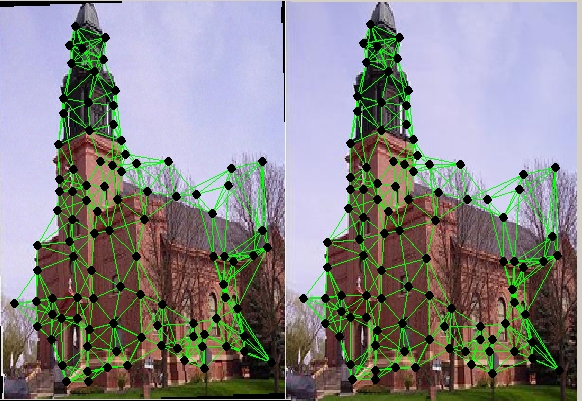
\includegraphics[scale=0.35]{fig/method2/test_imagetrafo1/initial_graphs.jpg} 
		\caption{Initial graphs on the lower level} 
	\end{subfigure}%% 
	\begin{subfigure}[b]{0.5\textwidth}
		\centering
		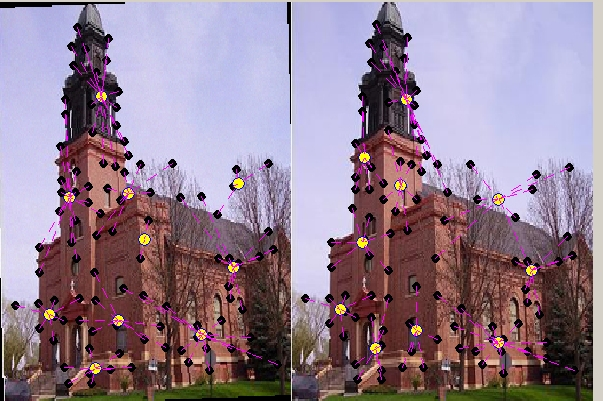
\includegraphics[scale=0.35]{fig/method2/test_imagetrafo1/initial_anchorgraphs.jpg} 
		\caption{Initial anchor graphs} 
	\end{subfigure} 
%	\caption{ Preprocessing}
%\end{figure}

%\begin{figure}[ht] 
	\begin{subfigure}[b]{0.5\textwidth}
		\centering
		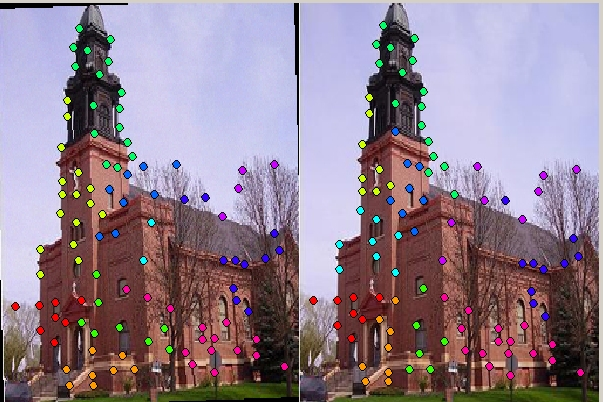
\includegraphics[scale=0.35]{fig/method2/test_imagetrafo1/partition_it1.jpg} 
		\caption{Iteration $1$: Graph Partition} 
	\end{subfigure}%% 
	\begin{subfigure}[b]{0.5\textwidth}
		\centering
		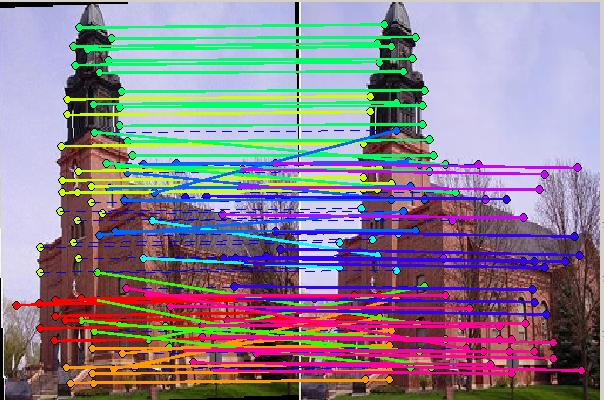
\includegraphics[scale=0.35]{fig/method2/test_imagetrafo1/LL_it1.jpg} 
		\caption{Iteration $1$: Graph Matching} 
	\end{subfigure} 
	\phantomcaption
%	\caption{Iteration $1$}
\end{figure}

\begin{figure}[ht] 
	\ContinuedFloat
	\begin{subfigure}[b]{0.5\textwidth}
		\centering
		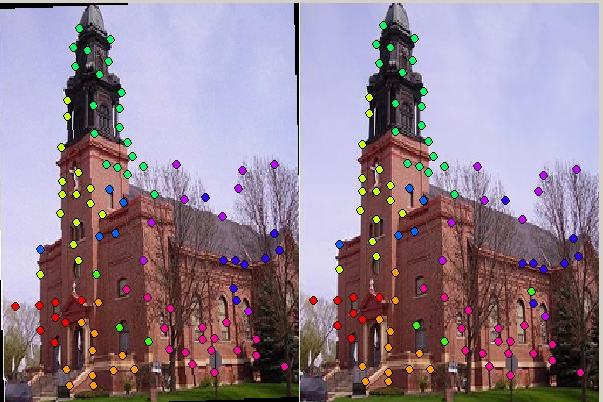
\includegraphics[scale=0.35]{fig/method2/test_imagetrafo1/partition_it6.jpg} 
		\caption{Iteration $6$: Graph Partition} 
	\end{subfigure}%% 
	\begin{subfigure}[b]{0.5\textwidth}
		\centering
		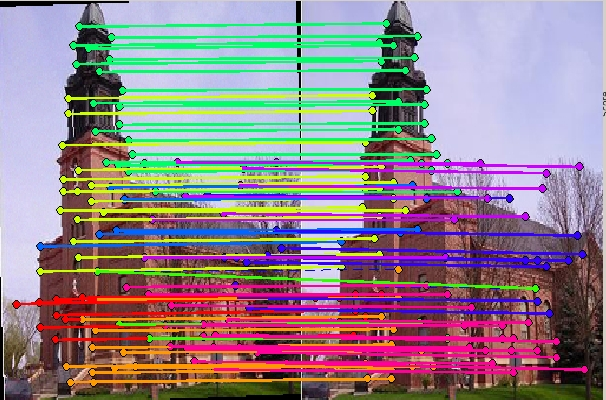
\includegraphics[scale=0.35]{fig/method2/test_imagetrafo1/LL_it6.jpg} 
		\caption{Iteration $6$: Graph Matching} 
	\end{subfigure} 
%	\caption{Iteration $6$}
%\end{figure}

%\begin{figure}[ht] 
	\begin{subfigure}[b]{0.5\textwidth}
		\centering
		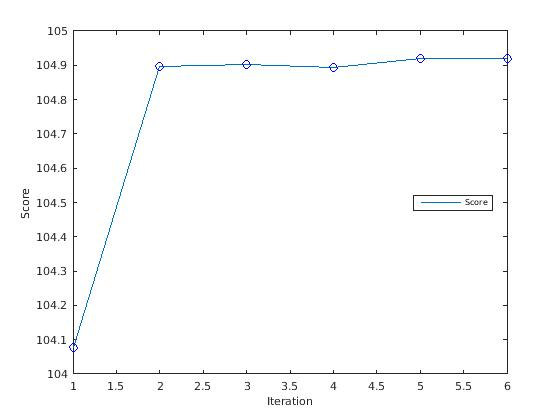
\includegraphics[scale=0.25]{fig/method2/test_imagetrafo1/score_HL.jpg} 
		\caption{Matching score on the Higher Level} 
	\end{subfigure}%% 
	\begin{subfigure}[b]{0.5\textwidth}
		\centering
		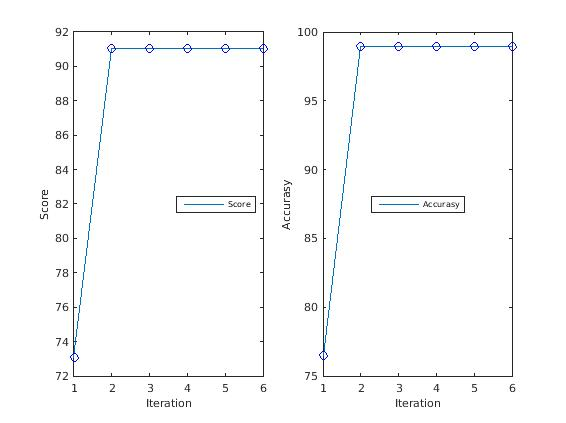
\includegraphics[scale=0.25]{fig/method2/test_imagetrafo1/accuracy_LL.jpg} 
		\caption{Matching score and accuracy on the Lower Level} 
	\end{subfigure} 
	\caption{Matching of the same images, rotation angle $\frac{\pi}{100}$}
%	\caption{Score and accuracy}
\end{figure}
\FloatBarrier

% ---------------------------------------
\subsubsection{Example $2$}
\begin{figure}[hbt] 
	\begin{subfigure}[b]{0.5\textwidth}
		\centering
		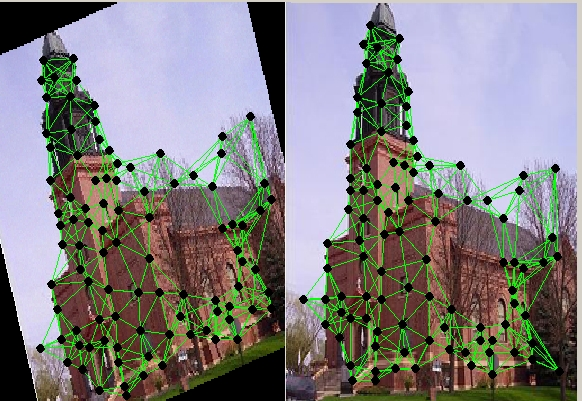
\includegraphics[scale=0.3]{fig/method2/test_imagetrafo2/initial_graphs.jpg} 
		\caption{Initial graphs on the lower level} 
	\end{subfigure}%% 
	\begin{subfigure}[b]{0.5\textwidth}
		\centering
		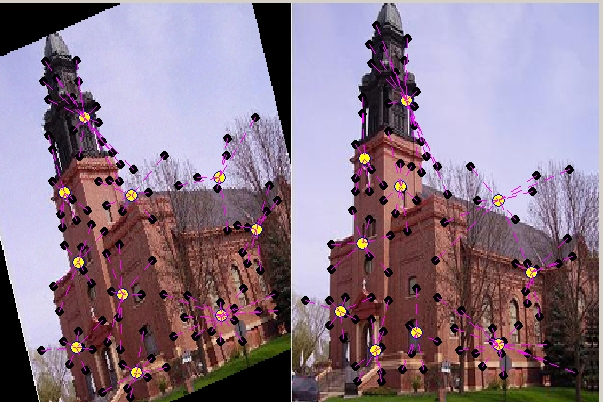
\includegraphics[scale=0.3]{fig/method2/test_imagetrafo2/initial_anchorgraphs.jpg} 
		\caption{Initial anchor graphs} 
	\end{subfigure} 
	%	\caption{ Preprocessing}
	\phantomcaption
	\end{figure}
	
	\begin{figure}[ht]
	\ContinuedFloat
	\begin{subfigure}[b]{0.5\textwidth}
		\centering
		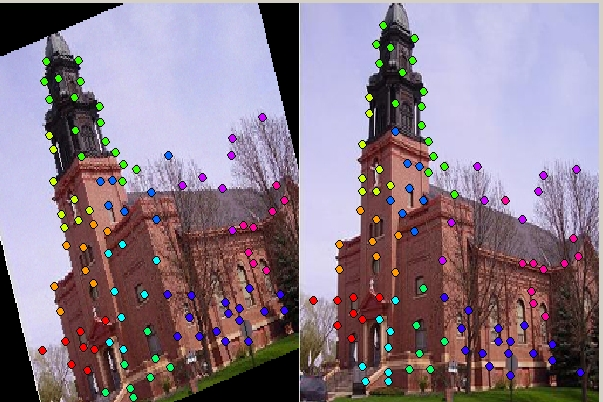
\includegraphics[scale=0.35]{fig/method2/test_imagetrafo2/partition_it1.jpg} 
		\caption{Iteration $1$: Graph Partition} 
	\end{subfigure}%% 
	\begin{subfigure}[b]{0.5\textwidth}
		\centering
		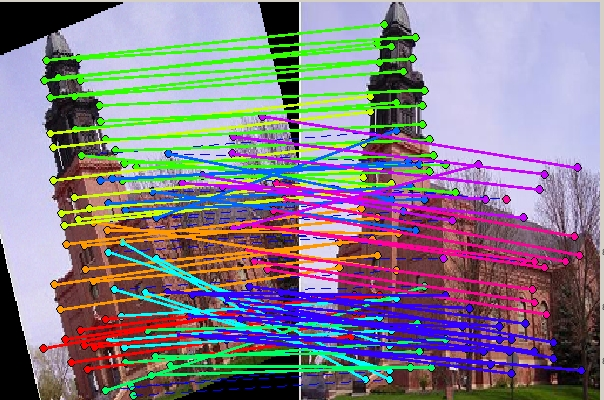
\includegraphics[scale=0.35]{fig/method2/test_imagetrafo2/LL_it1.jpg} 
		\caption{Iteration $1$: Graph Matching} 
	\end{subfigure} 
	%	\caption{Iteration $1$}
%	\end{figure}

%	\begin{figure}[ht] 
	\ContinuedFloat
	\begin{subfigure}[b]{0.5\textwidth}
		\centering
		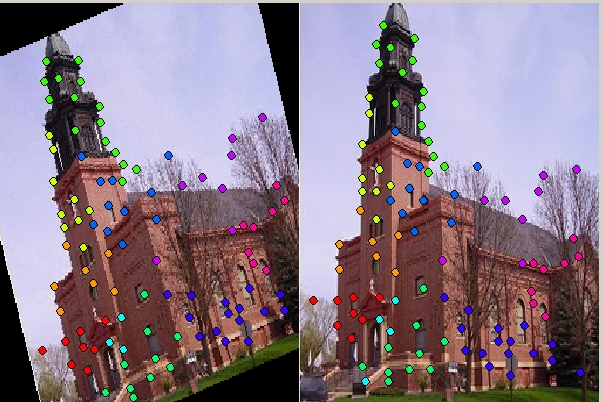
\includegraphics[scale=0.35]{fig/method2/test_imagetrafo2/partition_it2.jpg} 
		\caption{Iteration $2$: Graph Partition} 
	\end{subfigure}%% 
	\begin{subfigure}[b]{0.5\textwidth}
		\centering
		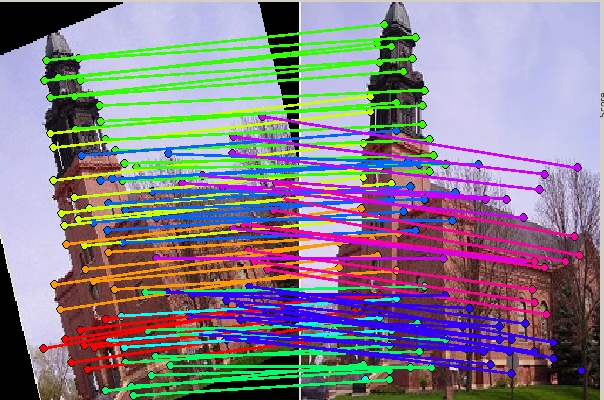
\includegraphics[scale=0.35]{fig/method2/test_imagetrafo2/LL_it2.jpg} 
		\caption{Iteration $2$: Graph Matching} 
	\end{subfigure} 
	%	\caption{Iteration $2$}
%	\end{figure}
	
%	\begin{figure}[ht] 
	\begin{subfigure}[b]{0.5\textwidth}
		\centering
		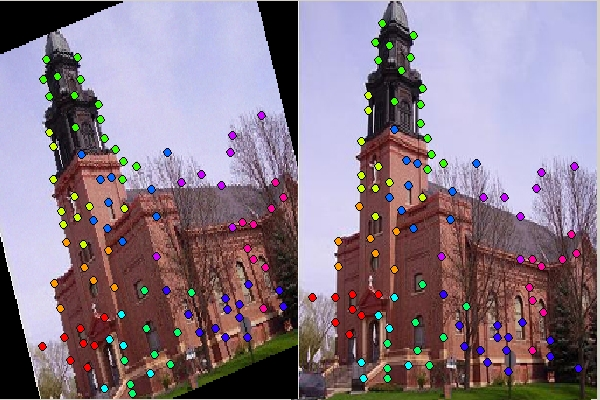
\includegraphics[scale=0.35]{fig/method2/test_imagetrafo2/partition_it11.jpg} 
		\caption{Iteration $11$: Graph Partition} 
	\end{subfigure}%% 
	\begin{subfigure}[b]{0.5\textwidth}
		\centering
		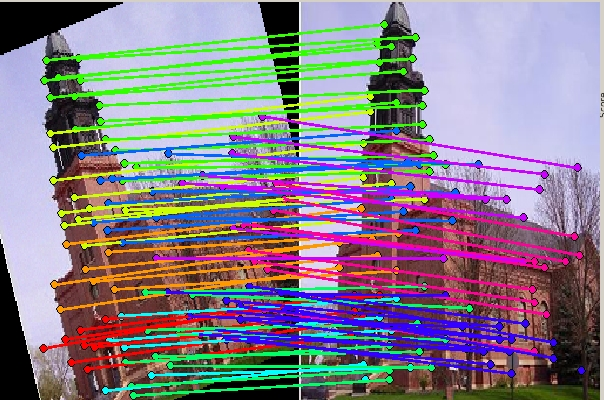
\includegraphics[scale=0.35]{fig/method2/test_imagetrafo2/LL_it11.jpg} 
		\caption{Iteration $11$: Graph Matching} 
	\end{subfigure} 
	%	\caption{Iteration $11$}
	\caption{Matching of the same images, rotation angle $\frac{\pi}{10}$}
	%\end{figure}	
	
	%\begin{figure}[ht] 
	\begin{subfigure}[b]{0.5\textwidth}
		\centering
		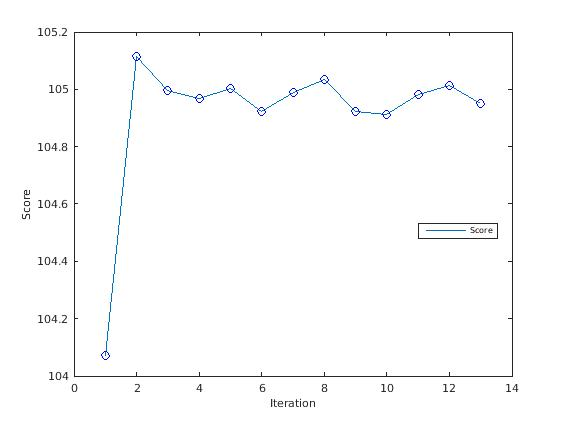
\includegraphics[scale=0.25]{fig/method2/test_imagetrafo2/score_HL.jpg} 
		\caption{Matching score on the Higher Level} 
	\end{subfigure}%% 
	\begin{subfigure}[b]{0.5\textwidth}
		\centering
		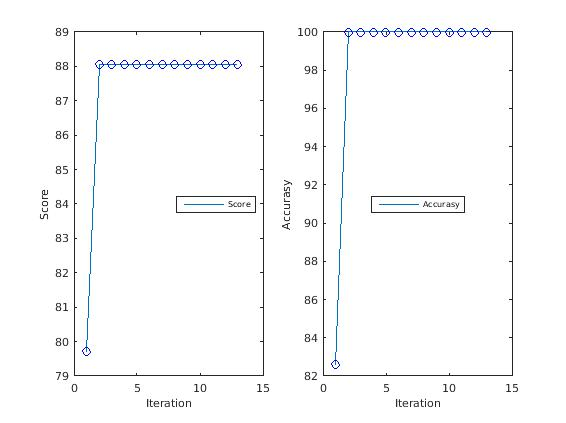
\includegraphics[scale=0.25]{fig/method2/test_imagetrafo2/accuracy_LL.jpg} 
		\caption{Matching score and accuracy on the Lower Level} 
	\end{subfigure} 
	%	\caption{Score and accuracy}
\end{figure}
\FloatBarrier
% ---------------------------------------

\subsubsection{Example $3$}

\begin{figure}[h] 
	\begin{subfigure}[b]{0.5\textwidth}
		\centering
		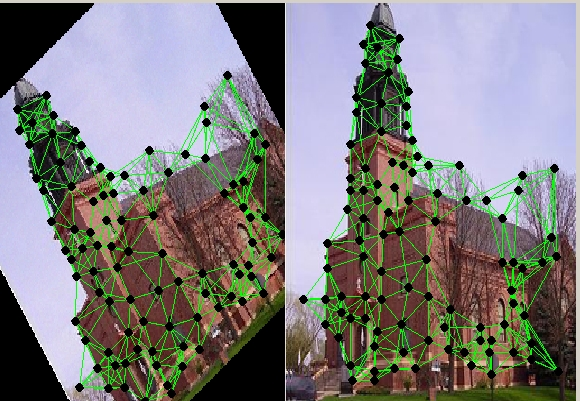
\includegraphics[scale=0.35]{fig/method2/test_imagetrafo3/initial_graphs.jpg} 
		\caption{Initial graphs on the lower level} 
	\end{subfigure}%% 
	\begin{subfigure}[b]{0.5\textwidth}
		\centering
		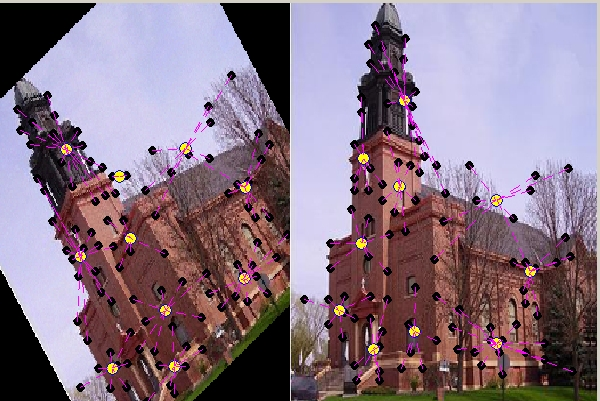
\includegraphics[scale=0.35]{fig/method2/test_imagetrafo3/initial_anchorgraphs.jpg} 
		\caption{Initial anchor graphs} 
	\end{subfigure} 
	%	\caption{ Preprocessing}
	%\end{figure}
	
	%\begin{figure}[ht] 
	\begin{subfigure}[b]{0.5\textwidth}
		\centering
		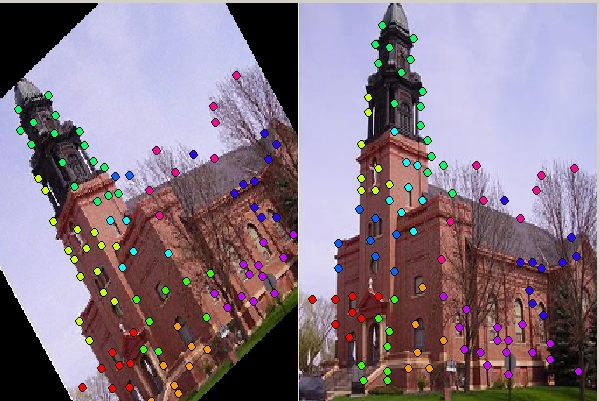
\includegraphics[scale=0.35]{fig/method2/test_imagetrafo3/partition_it1.jpg} 
		\caption{Iteration $1$: Graph Partition} 
	\end{subfigure}%% 
	\begin{subfigure}[b]{0.5\textwidth}
		\centering
		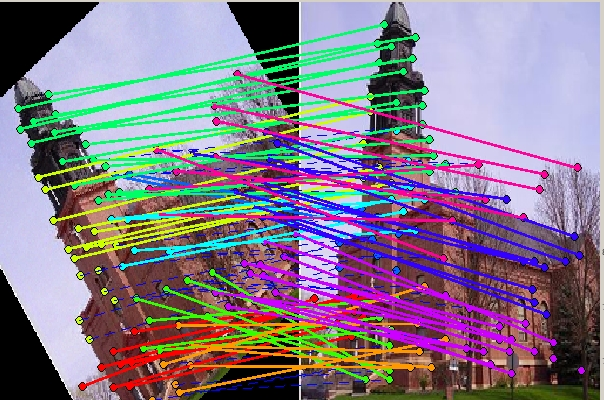
\includegraphics[scale=0.35]{fig/method2/test_imagetrafo3/LL_it1.jpg} 
		\caption{Iteration $1$: Graph Matching} 
	\end{subfigure} 
	%	\caption{Iteration $1$}
	%\end{figure}
	
	%\begin{figure}[ht] 
	\begin{subfigure}[b]{0.5\textwidth}
		\centering
		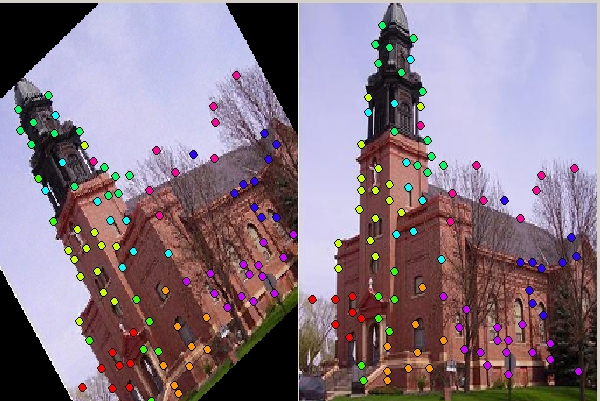
\includegraphics[scale=0.35]{fig/method2/test_imagetrafo3/partition_it12.jpg} 
		\caption{Iteration $12$: Graph Partition} 
	\end{subfigure}%% 
	\begin{subfigure}[b]{0.5\textwidth}
		\centering
		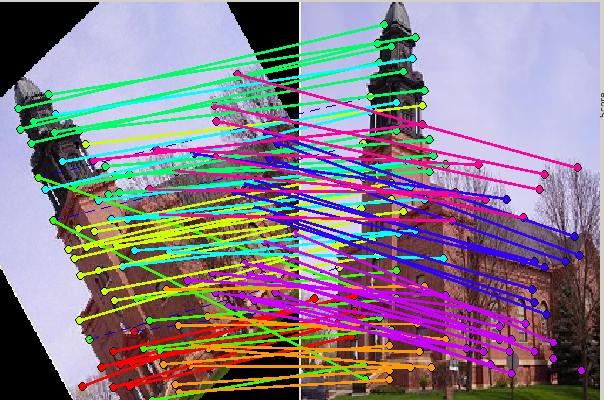
\includegraphics[scale=0.35]{fig/method2/test_imagetrafo3/LL_it12.jpg} 
		\caption{Iteration $12$: Graph Matching} 
	\end{subfigure} 
	%	\caption{Iteration $12$}
	\phantomcaption
	\end{figure}
	
	\begin{figure}[h] 
	\begin{subfigure}[b]{0.5\textwidth}
		\centering
		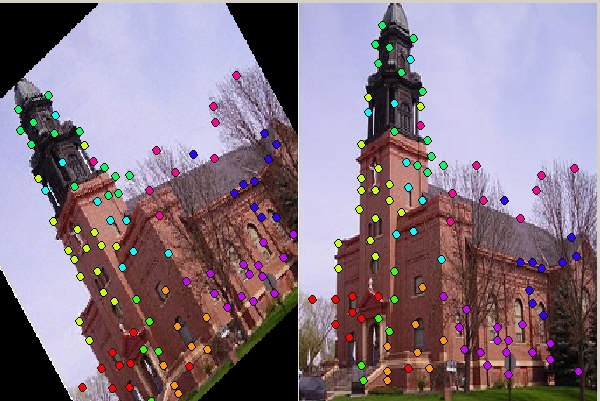
\includegraphics[scale=0.35]{fig/method2/test_imagetrafo3/partition_it13.jpg} 
		\caption{Iteration $13$: Graph Partition} 
	\end{subfigure}%% 
	\begin{subfigure}[b]{0.5\textwidth}
		\centering
		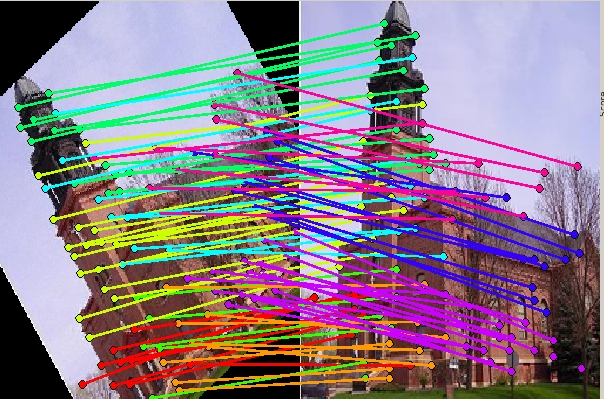
\includegraphics[scale=0.35]{fig/method2/test_imagetrafo3/LL_it13.jpg} 
		\caption{Iteration $13$: Graph Matching} 
	\end{subfigure} 
	%	\caption{Iteration $13$}
%	\end{figure}
	
%	\begin{figure}[h] 
	\begin{subfigure}[b]{0.5\textwidth}
		\centering
		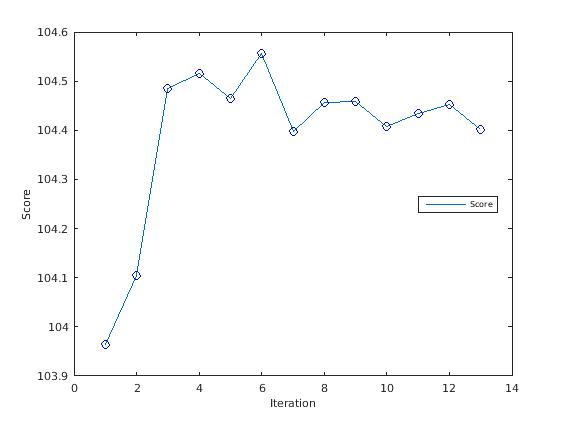
\includegraphics[scale=0.25]{fig/method2/test_imagetrafo3/score_HL.jpg} 
		\caption{Matching score on the Higher Level} 
	\end{subfigure}%% 
	\begin{subfigure}[b]{0.5\textwidth}
		\centering
		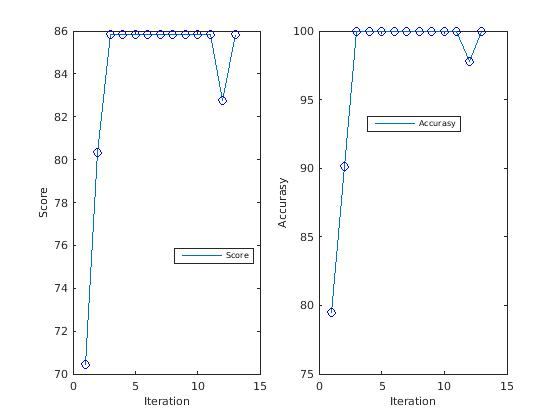
\includegraphics[scale=0.25]{fig/method2/test_imagetrafo3/accuracy_LL.jpg} 
		\caption{Matching score and accuracy on the Lower Level} 
	\end{subfigure} 
	%	\caption{Score and accuracy}
	\caption{Matching of the same images, rotation angle $\frac{\pi}{5}$}	
\end{figure}
\FloatBarrier
% ------------------------------------------------------------------------------------------------------------
% ---------------------------------------        Bibliography
\bibliographystyle{abbrv}
\bibliography{bibliography}
	
\end{document}